\documentclass{article}
\usepackage[utf8]{inputenc}
\usepackage{amsmath}
\usepackage[magyar]{babel}
\usepackage{amsfonts}
\usepackage{MnSymbol}
\usepackage{wasysym}
\usepackage{graphicx}




\title{Osztott rendszerek specifikációja és implementációja - dokumentáció}
\author{Lombosi Balázs - D3BA80}
\date{\today}

\begin{document}
\maketitle

\tableofcontents
\newpage

\section{Feladat}

A bemenet --input.txt -- első sorában tartalmazza az $n$ pozitív egész számot, következő $n$ sorában pedig a hallgatók neptun kódját.
$n$\\
$Neptun_{1}$ - az 1. hallgató neptun kódja \\
$\dots\\ $
$\dots\\ $
$Neptun_{n}$ - az n. hallgató neptun kódja \\

A program olvassa be az adatokat, majd rendezze az adatokat növekvő sorrendbe párhuzamosan, $MergeSort$ rendező algoritmus segítségével.
Az az eredményt írja az -- output.txt -- kimeneti fájlba.
Megkötés, hogy a fájlból olvasást és a fájlba írást egy szál/folyamat végezze, és a $MergeSort$ algoritmus két ágához mindig új folyamat induljon.
\newpage

\section{Felhasználói dokumentáció}

\subsection{Környezet}
A program több platformon futtatható, nincsen dinamikus függősége. Telepítésre nincs szükség, elegendő a futtatható állományt elhelyezni a számítógépen \\
(Windows operációs rendszeren \textit{.exe} fájl, UNIX operációs rendszeren \textit{.out} fájl).

\subsection{Használat}
A program használata egyszerű, mert nem vár parancssori paramétereket, így akár parancssoron kívül is lehet futtatni. A fájl mellett kell elhelyezni az \textit{input.txt} fájlt melyet a program beolvas, az eredményt pedig az \textit{output.txt} nevű fájlba írja, a játékok neve alapján betűrendben.\\
A program futásának feltétele, hogy a bemeneti fájl \textit{(input.txt)} felépítése helyes legyen, azaz a feladatban leírtak szerint legyenek benne az adatok.
\newpage

\section{Fejlesztői dokumentáció}
\begin{itshape}
A feladat megoldásához a C++11 es szabványt választottam és annak beépített nyelvi elemeit. \\
\end{itshape}

\subsection{A megoldás módja}
A kódot logikailag több részre bonthatjuk, egy fő- és több alfolyamatra. A főfolyamat, a $main()$ függvény lesz felelős az adatok beolvasásáért az input fájlból, ami most az \textit{input.txt}. A folyamat a beolvasáskor egy $vector$ adatszerkezetet tölt fel az adatokkal, a főfolyamat ezek után elindítja a $merge_sort$ folyamatot a teljes vektorral. A $merge_sort$ rekurzívan további $merge_sort$ folyamatokat indít a teljes vektor rész sorozataival.
\subsection{Implementáció}
A C++ beépített adatszerkezeteiből  az adatok tárolásához az $std::vector$-t. Pontosabban, a beolvasott adatokat egy $std::vector<std::string>$ adatszerkezetben tároljuk.

A párhuzamosságot a C++11 szabvány nyelvi elemeit kihasználva valósítjuk meg. Az eredmény helyben, a beolvasott vektorban lesz.

A \textit{merge\_sort} algoritmus a több elemből álló vektorokat kisebb rész sorozatokra bontja. És ezeket a kisebb rész sorozatokat fogja a $merge$ függvény összefésülni rendezett formába, abban az esetben ha a részsorozat hossza nagyobb mint egy küszöb szám, ezt a küszöbszámot a 3.2.1es fejezetben részletezzük. Abban az esetben ha a részsorozat hossza kisebb mint a küszöb szám buborék rendezést alkalmazunk.

A $merge$ függvény paraméterül kapja az adott részsorozatot. A kapott részsorozatot újabb két részsorozatra bontja, és amíg egyik részsorozat se üres, az első elemeket összehasonlítja és a kisebbet beleteszi egy vektorba majd a kisebb értékkel rendelkező iterátort lépteti így kapunk az iteráció végén egy rendezett sorozatot.

A teljes implementáció egyetlen forrásfájlba szervezve, a $main.cpp$ fájlban található meg.
\newpage
\subsubsection{Küszöbszám}
A rendezés, gyorsításához a rekurziót nem hagyjuk, hogy addig fusson amíg egy elem marad hanem ehhez egy küszöbszámot alkalmazunk, ami alatt a buborék rendezés, gyorsabb mint a sorozat feldarabolása és összefésülése, mérések alapján ez a küszöb szám 300 körülre tehető. Azaz, ha egy sorozatnak 300 eleme van gyorsabb a buborék rendezés mint a sorozat további darabolása és összefésülése. A méréshez az 
\textit{input\_3.txt} fájlt, használtam fel ahol $10000$ elem található .A küszöbszám meghatározásához használt mérések grafikonja.
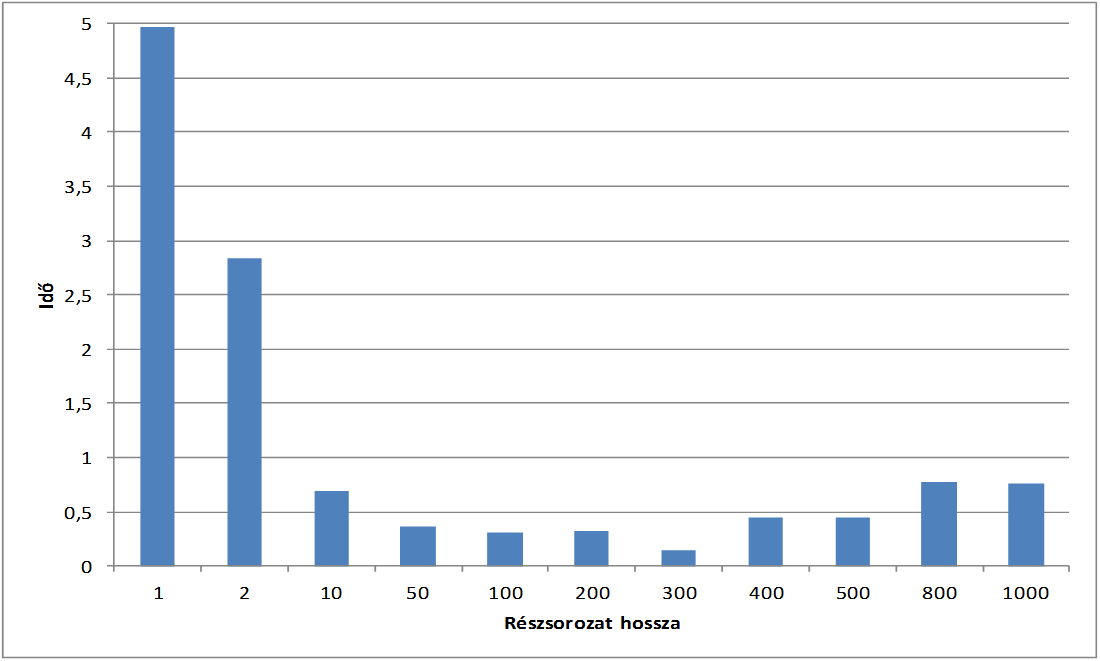
\includegraphics[scale=0.42]{meresek}
\subsection{Fordítás}
A program forráskódja a $main.cpp$ fájlban található.
A program fordításához követelmény egy C++11 szabványt támogató fordítóprogram megléte a rendszeren. A legnépszerűbbek az $msvc$, $g++$ és $clang$.
A fordítás menete (UNIXon g++ 4.9.2-es verziójú fordítóval, Windowson g++ 5.1.0 verziója fordítóval lett tesztelve):
\begin{itemize}
	\item UNIX környezetben a következő: $'g++ \; -std=c++11 \; main.cpp -lpthread'$,
	\item Windows környezetben: $'g++ \; -std=c++11 \; main.cpp'$ .
\end{itemize}
Az $-std=c++11$ kapcsoló szükséges, mert alapértelmezetten egy régebbi C++ szabványt támogat a fordító. UNIX környezetben szükséges a -pthread vagy -lpthread kapcsoló, hogy a fordító tudja, hogy többszálú programot fordít.

\subsection{Tesztelés}
A programot a megadott teszt input fájlokkal teszteltem le. A teszteléshez használt processzor: Intel Core i7-3632QM @ 2.20Ghz .\\

\end {document}